% !TEX root = ../../ozan_sener_thesis.tex
\label{intro}
Understanding humans is an important skill for robots working with humans. Robots not only need to detect the activity and pose of the human but also need to anticipate \emph{what activities can a human possibly perform in the near future in which poses} in order to choose the right actions. Anticipation ability is especially important for assistive robots, and we have recently seen many successful collaborative robotics applications \cite{collob1,collob2,hemaISER} using the most likely action(s) humans might take in near future. Although existing methods can successfully detect most likely activity and/or human pose, robots need to model uncertainty as well. In this chapter, we focus on estimating the set of all possible future states with their likelihoods.

%For example, Koppula et al. \cite{hemaAnt} used anticipation in assistive robotic setting and successfully \emph{opened doors} and \emph{served drinks} by reacting to possible future human actions.

Anticipation is a challenging task, and it requires us to model the relationships between several objects and the human(s) in the scene, as well as their temporal evolution. Although the modelling assumptions and model parametrization varies, the common approach \cite{hemaAnt,gpcrf,hemaECCV,tian} is using Conditional Random Field (CRF) to represent the rich relations in the scene, and anticipating a single or a few most likely future states. Since the future is ambiguous, the most likely state might not be sufficient enough to assess the risk of each action. For example, consider a collaborative cooking scenario, the object that human is reaching is typically a distribution over many objects. Computing the trajectory, that is least likely to conflict with the human, is only possible via consideration of all future possibilities. The question, we address in this chapter, is: \emph{How can we estimate all plausible future activities and their probabilities in a scene modelled by a CRF?}

%Moreover, we call these probabilities as a \emph{belief}.
%Since we focus on finding all plausible future actions and their respective probabilities, we study the limitations of CRFs in such a setting
%A standard approach for anticipating future human activities is modelling the rich relationships in the scene by using Conditional Random Fields (CRFs). Moreover,
%Moreover, detecting the activity human is performing
%not only needs to understand the activity a human is performing, but also need to perform reactive responses.
%Consider the applications of surveillance and  robotics, where given an input video, one
 %For example, an alert may need to be issued in the case of surveillance or a reactive action may need to be taken by a robot in the case of co-robot scenario.
%Anticipation of the possible human activities is a challenging task and it require us to model the


% A standard approach is to use a Conditional Random Field (CRF) to represent the relations between the objects, human(s) and activities \cite{hemaIJRR,hemaAnt}.  %In general, it is possible to obtain the maximum a posteriori (MAP) solution over a CRF to find most likely future action(s).

 %However, a robot needs more than the most likely state(s) in order to make a decision. Robot needs all plausible futures with their corresponding belief values. For example, a plausible but less likely future might require taking precautions like getting close enough to react.



%A recent work \cite{embr,divmbest}, empirically computes modes of the CRF likelihood by relying on diverse samples. While this work does not apply directly to estimating beliefs in a Bayesian filtering setting,  We use the diverse sampling ideas for efficient inference in our model (see Section~\ref{relwork} for more details).

\begin{figure}[t]
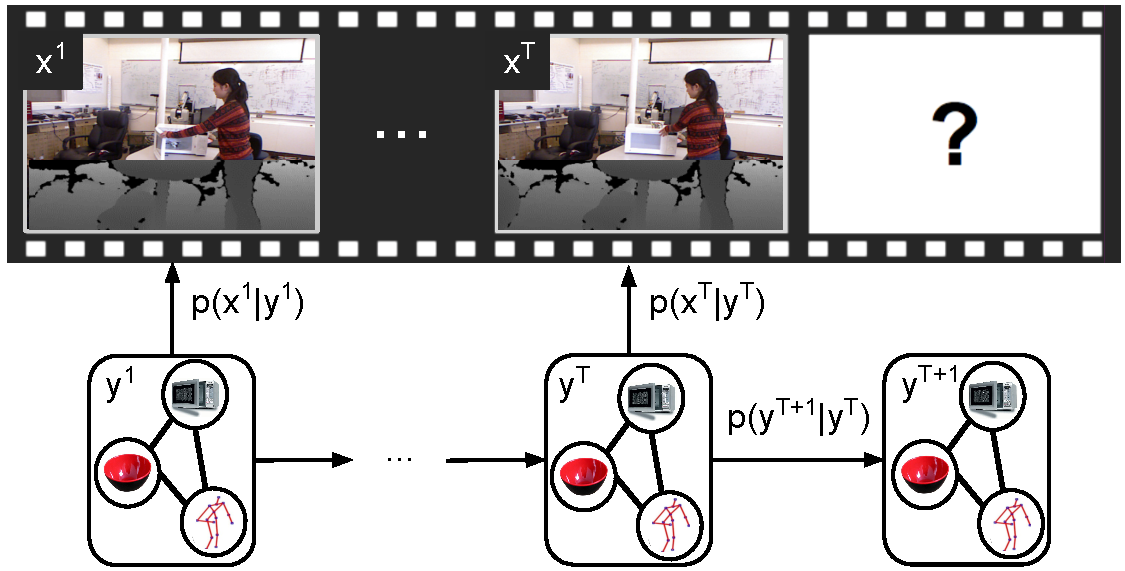
\includegraphics[width=\textwidth]{Fig1}
\caption{Figure is showing the state and measurements at each time represented by a CRF.
Our algorithm, rCRF, enables the application of recursive Bayesian estimation to CRF-based scene models. rCRF computes the full belief over human activity and object affordances ($y^1,\ldots,y^{T+M}$) by using RGB-D Video ($x^1,\ldots,x^T$).}
% In order to so, we propose a new model, rCRF, which can jointly use bayesian filtering and CRFs.}
%  which are not observed.}
%Estimating the belief over a CRF and using the estimated belief for anticipation and robot planning. \emph{(Colors of the nodes are representing the labels.)}}
\label{fig1}
\end{figure}

% modeling temporal evolution is still challenging in such a setting since the sampling procedure does not use temporal information \emph{(see Section~\ref{relwork} for mote details on this challenge)}.
Bayesian filtering methods can accurately estimate a belief (set of probabilities) over variables of interest from sequential data. However, it is still very challenging to estimate a belief over a CRF for two reasons. Firstly, it is not tractable to enumerate the labels over a CRF model since the output space has a dimension exponential in the number of objects, labels, and the temporal length\footnote{Typically with 10 objects, 10 min. length (with 1 sec. long segments), 10 activity and 10 object labels, dimension is $(10^{10}\times10)^{10\times60}=10^{6600}$.}. Secondly, there is a modelling difference between CRFs and Bayesian filtering framework. CRF is based on a discriminative setting whereas the Bayesian filtering mostly relies on the generative formulation.
% that requires the conditional probability of the observation given the variables of interest.
%where it models the conditional probability of the variables of interest given an observation,

In this chapter, we present a recursive algorithm -- Recursive CRF (rCRF) -- which can efficiently estimate a full belief over a CRF-based temporal scene model. rCRF can be seen as an efficient belief estimation method which enables us to use CRF-based scene model in Bayesian filtering. It models the temporal evolution via Bayesian updates and models the measurements in the scene via CRF. In order to use CRFs in such a scenario, we solve two problems. First, we present an approximation to convert the discriminative likelihood of the CRF into a generative measurement equation. Second, we use structured diversity for tractable computation. To the best of our knowledge, rCRF is the only tractable method that can use a CRF-based scene model in a recursive Bayesian filtering.
%Since we define the belief function recursively, we iterate the message propagation and diverse sampling until the convergence.

We apply the rCRF to the problem of activity detection and anticipation from RGB-D data. As a CRF-based scene model, we use the model from \cite{hemaIJRR} which represents the scene as a CRF over human activity and object affordances. We then use the RGB-D video to detect and anticipate activities via rCRF. %We use the rCRF framework in order to anticipate the future activities as well.

Our experiments show that we outperform the state-of-the-art methods for detection and anticipation, and the improvement in the anticipation accuracy is significant. In addition to the improvements in accuracy, we show that our anticipation also improves the computation time and runs near real-time.

%We believe that the presented efficient and accurate estimation of a full belief can be combined with an optimal decision mechanisms (e.g. minimum Bayes risk \cite{decisionTheory,nabbe2007extending}) for better assitive robots.

In summary, the contributions of this work are:
\begin{itemize}
\item  We present Recursive-CRF (rCRF) method that uses the rich modeling power of CRF in
Bayesian filtering setting.
%  allows CRF-based scene models in a Bayesian filtering.
% \item  We present a recursive method in order to estimate the full belief over an rCRF.
\item  We present a structured-diversity based approach to enable tractable computation of the belief.
\item  We apply our rCRF method to the problem of activity detection and anticipation in
RGB-D videos.
%\item  Our experiments show that rCRF significantly outperforms the state-of-the-art methods, both in accuracy and inference time.
\end{itemize}
